\chapter{Applications}\label{cap:5}


{\lettrine[loversize=0.25,findent=0.2em,nindent=0em]{T}{ODO} 

\subsection{Logistic Map}

The next two examples show how the algorithms fare when modeling a system whose PFSA is unknown or non-existent. A sequence from these systems will be analyzed and a PFSA model will be created and its output will be compared to the original sequence to see how well this Markovian model approximates a dynamic system which might not even be Markovian.

The first of these examples is the Logistic Map, a symbolic dynamic system whose outputs is given by the difference equation \cite{asok.14}:

\begin{equation}
x_{k+1} \triangleq rx_k(1-x_k), \label{eq:logisticmap}
\end{equation}


\noindent which shows chaotic behavior when the \textit{r} parameter is approximately 3.57. As in \cite{asok.14}, the initial x is set to 0.5 and \textit{r} = 3.75. A sequence of length $10^{-7}$ was generated from this equation and then it was quantized with a ternary alphabet: values x$_k \leq 0.67$ were mapped to 0; when 0.67 < x$_k \leq 0.79$, it was mapped to 1 and when x$_k$ > 0.79 it was mapped to 2. A part of that sequence and the specified threshold are shown in Figure \ref{fig:lmapseq}.

\begin{figure}
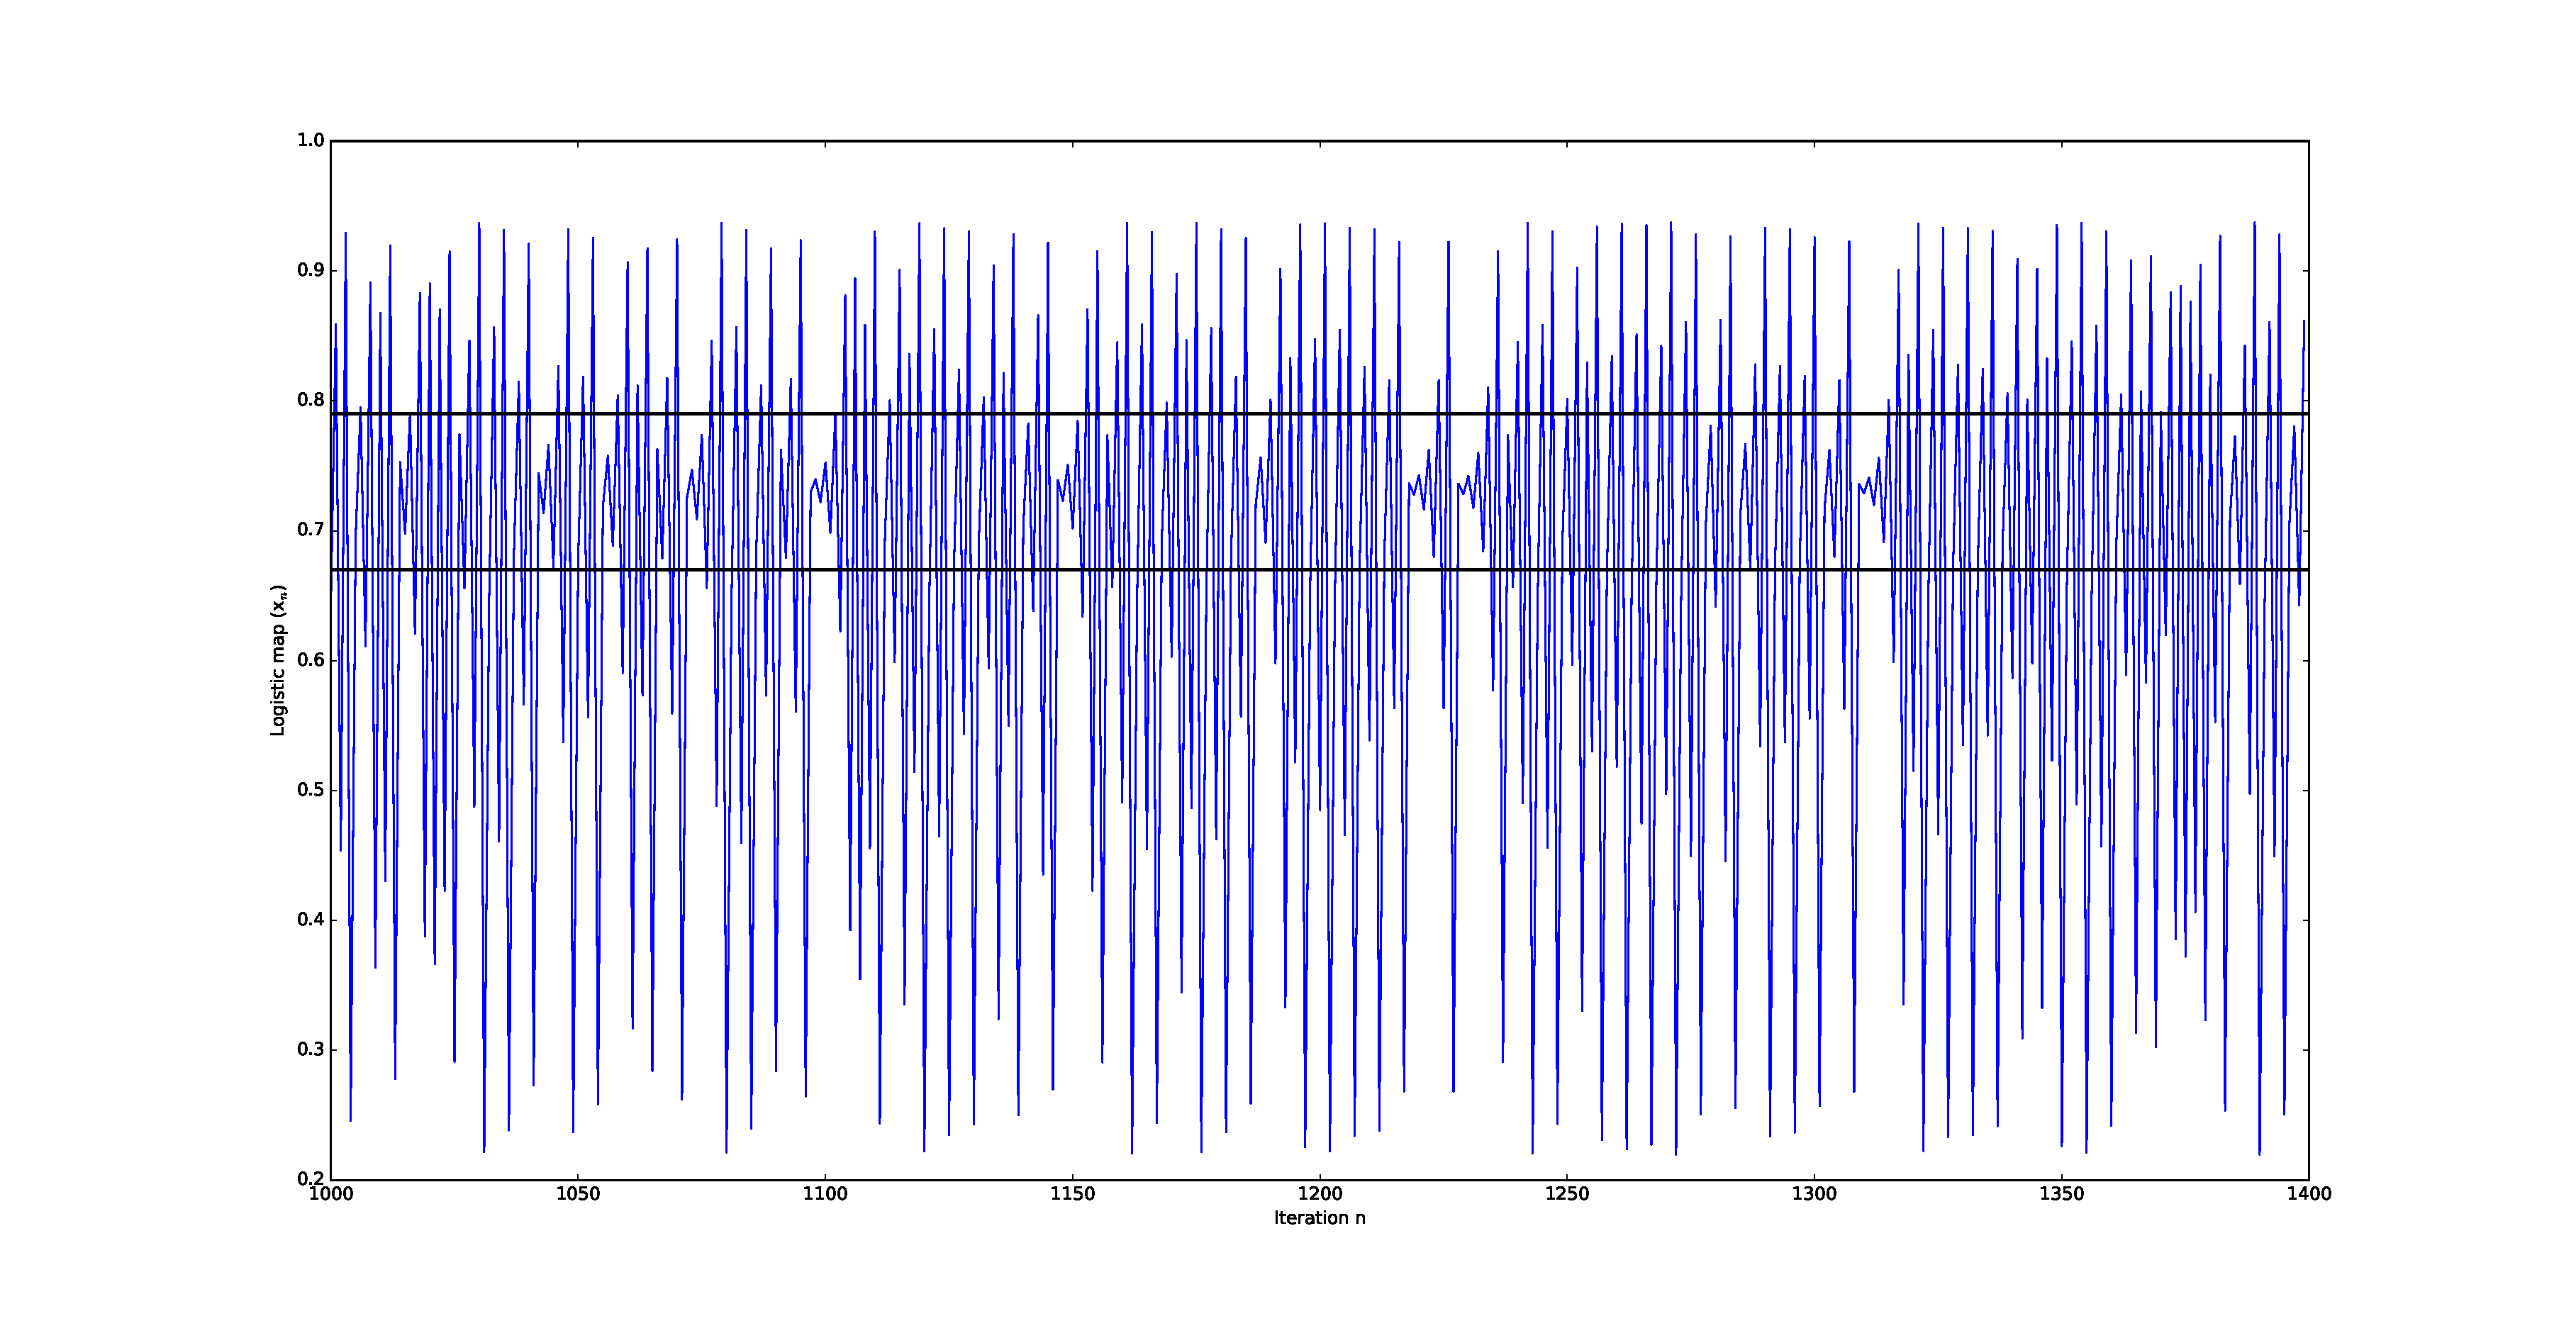
\includegraphics[scale=0.25]{Figuras/logisticmap.eps}
\caption{Part of the Logistic Map generated by Equation \ref{eq:logisticmap} with x$_0$ = 0.5 and $r$ = 3.75.\label{fig:lmapseq}}
\end{figure}

From this ternary sequence, the three algorithms were applied in order to obtain a Markovian model for the logistic map. As seen in Table \ref{tab:lmapsynch}, two sets of synchronization words were found for the sequence, one for each of the confidence levels used in the algorithm. For $\alpha = 0.95$, the synchronization words are 2, 00, 01, 10 and 11. On the other hand, for $\alpha = 0.99$, the synchronization words are 2, 00, 01, 10 and 111. The higher value of $\alpha$ made 11 be discarded as synchronization word candidate and allowed 111 to be tested. With the lower value, 11 was never discarded and 111 could not achieve candidate status.

\begin{table}
\centering
\caption{Synchronization Words for the Logistic Map Ternary Sequence. \label{tab:lmapsynch}}
\begin{tabular}{|l|c|c|}
\hline
 & \multicolumn{2}{c|}{\textbf{$\alpha$}}\\
 \hline
\textbf{W} & 0.95 & 0.99 \\
\hline
2 & 2 & 2 \\ 
3 & 2, 00, 01, 10, 11 & 2, 00, 01, 10 \\ 
4 & 2, 00, 01, 10, 11 & 2, 00, 01, 10, 111 \\ 
5 & 2, 00, 01, 10, 11 & 2, 00, 01, 10, 111 \\
6 & 2, 00, 01, 10, 11 & 2, 00, 01, 10, 111 \\ 
7 & 2, 00, 01, 10, 11 & 2, 00, 01, 10, 111 \\ 
 \hline
\end{tabular}
\end{table}

\subsection{Gilbert-Elliot Channel}

The Gilbert-Elliot Channel (GEC) is used to model digital communication channels that suffer with burst errors, i.e. a channel that usually has low probability of error but that has moments where many sequential errors occur. As described in \cite{mushkin.89}, Figure \ref{fig:gec} is the GEC model. It operates in two states, \textit{0} (the "good channel") and \textit{1} (the "bad channel"). While it is in \textit{0}, it works as a Binary Symmetric Channel (BSC) with error probability of $p_0$, which is usually very small, indicating a state in which the channel does not produce too many errors. When it is in state \textit{1}, it is a BSC with error probability $p_1$ which is higher than $p_0$, indicating a state where it is more probable for an error to occur. When in state \textit{0}, it has a probability $q$ of transitioning to state \textit{1} and $1-q$ to stay in \textit{0}. Similarly, when in \textit{1}, it transitions to \textit{0} with probability $q$ and stays with probability $1-q$. This indicates that there is a chance from going to one situation to the other.

\begin{figure}
\centering
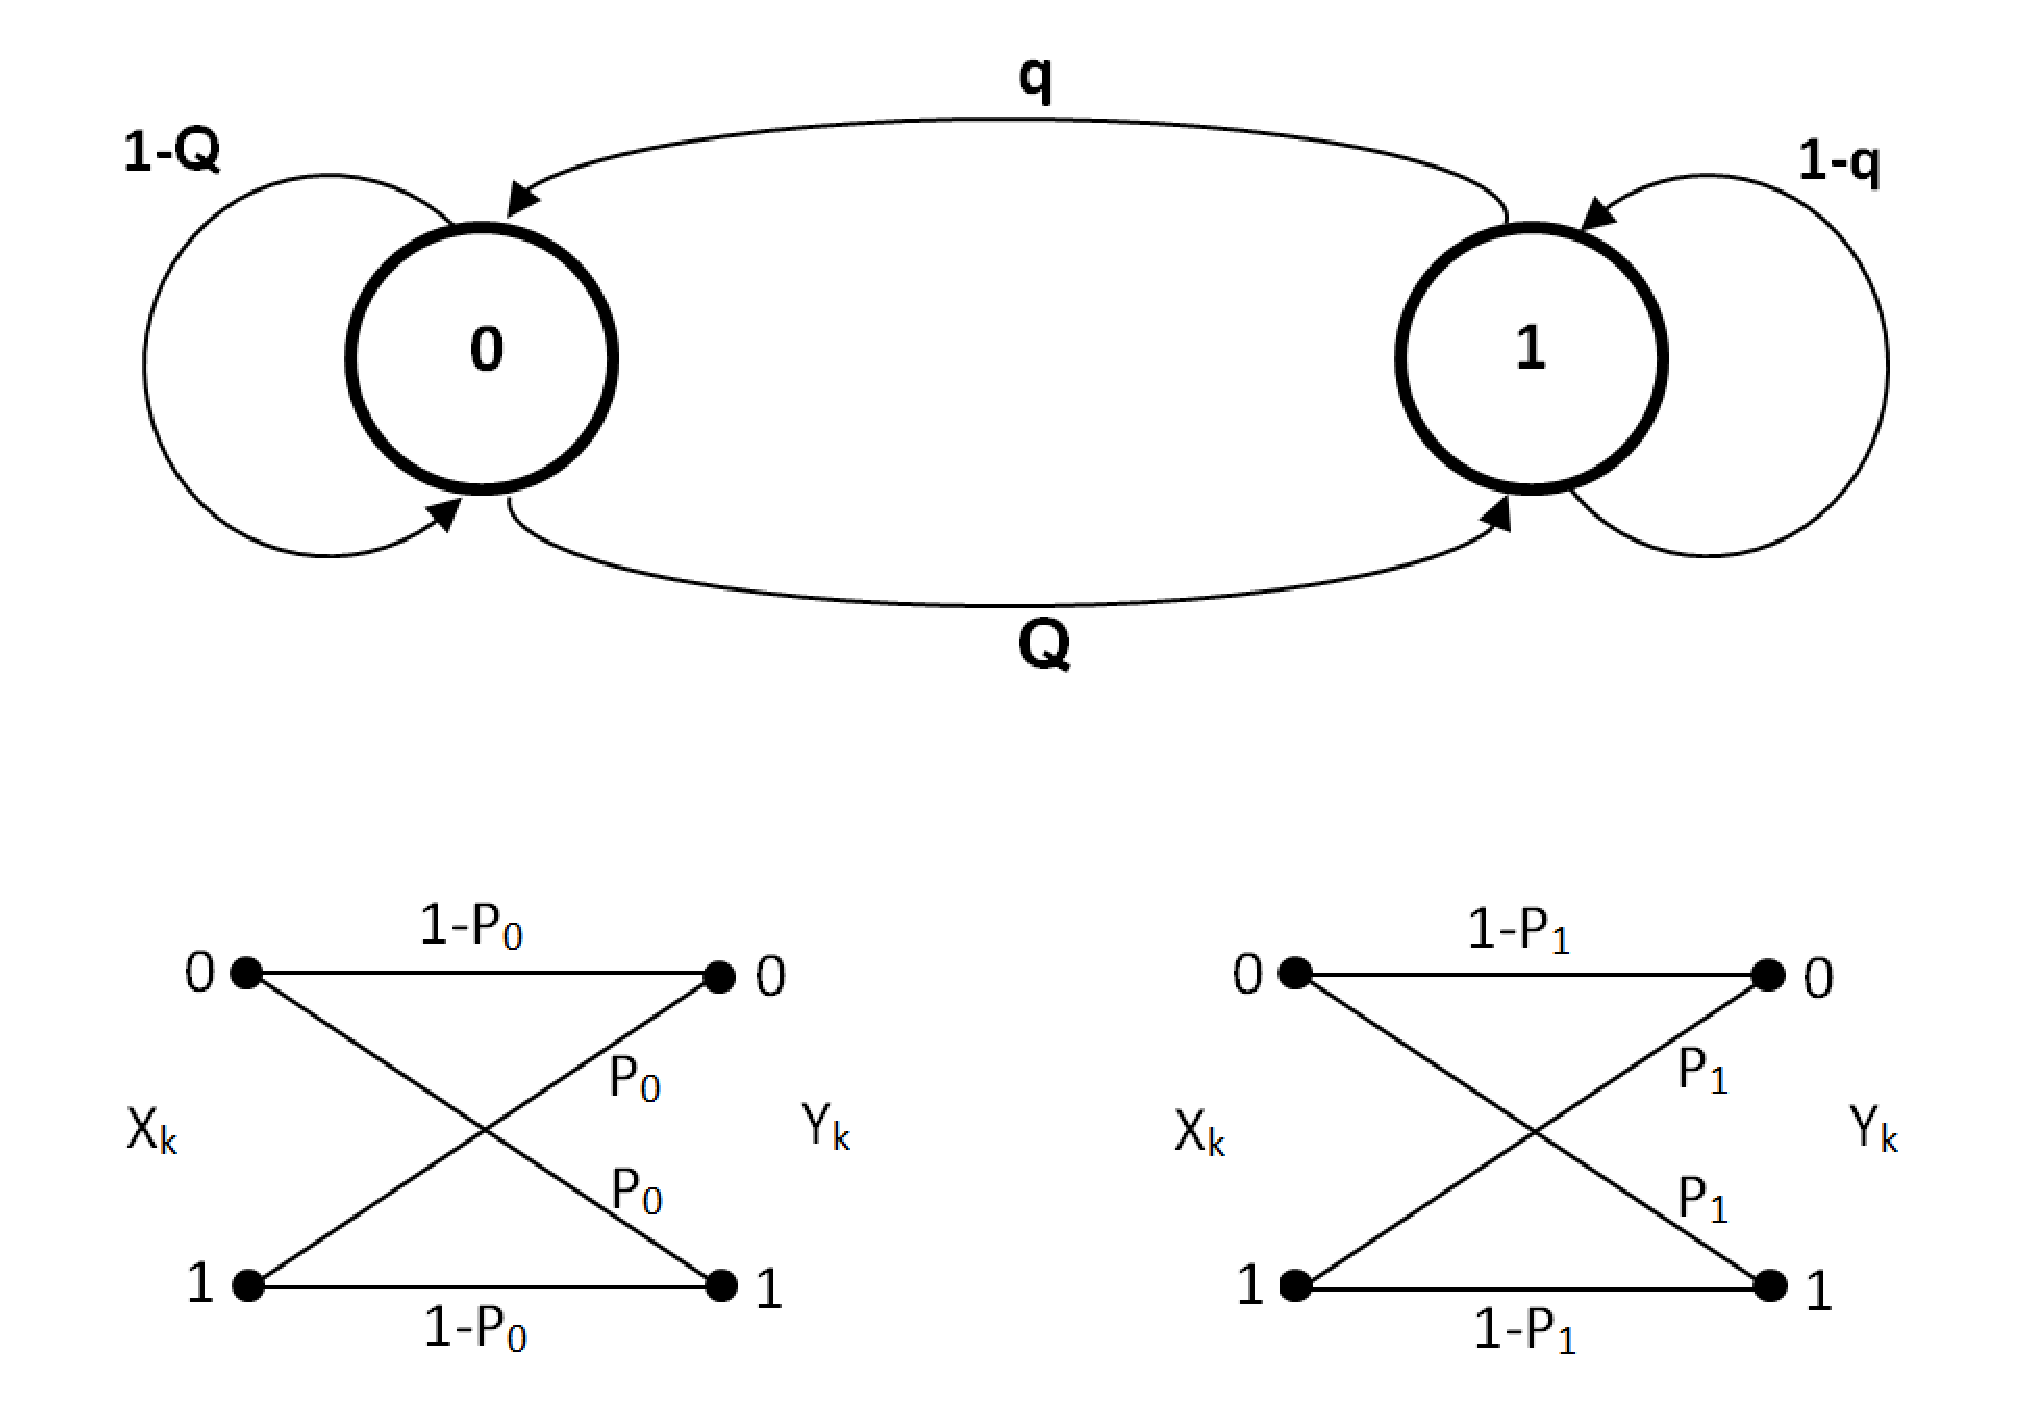
\includegraphics[width=8cm, height=6cm]{Figuras/figgec.eps}
\caption{\label{fig:gec} The Gilbert-Elliott Channel.}
\end{figure}

Other important parameters of the GEC that need to be evaluated are its memory $\mu$ and the Bit Error Rate (BER), which is a percentage of errors in the transmission. The memory $\mu$ is defined as:

\begin{equation}
\mu = 1 - q - Q. \label{eq:mumemory}
\end{equation}

\noindent which reduces to a memoryless BSC when $\mu = 0$. This parameter is called memory because, as seen in \cite{mushkin.89}, the GEC's autocorrelation function is:

\begin{equation}
R_{GEC}[m] = (\text{BER})^2 +\frac{Qq(p_1-p_0)²}{(q+Q)²}(1-q-Q)^m, \label{eq:rgec}
\end{equation}

\noindent which, without getting into much detail, shows that $\mu$ influences how a symbol is related to another one that is $m$ symbols apart. The BER is given by:

\begin{equation}
\text{BER} = \frac{q}{q+Q}p_0 + \frac{Q}{q+Q}p_1. \label{eq:gecber}
\end{equation}

The GEC can be designed to obtain specific values of $\mu$ and BER and then it is possible to compare how close to the design parameters the generated PFSA are able to get in order to evaluate their performance.

A binary sequence going through this channel would be output in instant $k$ the following way:

\begin{equation}
y_k = x_k\oplus z_k, \label{eq:binarychannel}
\end{equation}


\noindent in which $x_k$ is the input symbol at instant $k$, $z_k$ is the error symbol at instant $k$ and $\oplus$ is binary addition operation. When $z_k$ is 0, $y_k$ will be equal to $x_k$, which means that no error occurred. On the other hand, when it 1, $y_k$ will be $x_k \oplus 1 = \neg x_k$, indicating the occurrence of an error. The symbol $z_k$ has a probability $p_e$ of being 1 and $1-p_e$ of being 0 and $p_e$ is equal to $p_0$ if the channel is in state \textit{0} and equal to $p_1$ when it is in state \textit{1}. Following this rule, an error sequence $z$ can be generated to model how the channel and how it affects an input sequence. An error sequence of length $10^{7}$ is generated and used as input to the algorithms. The GEC is strictly not Markovian and this is an example to show how the algorithms fare in modeling such a system in a Markovian fashion.